\documentclass[14pt,handout,utf8]{beamer}
%\setlength{\paperwidth}{297mm}
%\setlength{\paperheight}{210mm}
%\usepackage[scale=0.78,size=a1]{beamerposter}
\usepackage[scale=1.0,size=a4,orientation=portrait]{beamerposter}
%\setlength{\topmargin}{20mm}
\setbeamersize{text margin left=10mm,text margin right=10mm}

\usepackage{cmap}
\usepackage[T1,T2A]{fontenc}
\usefonttheme[onlymath]{serif}
\usepackage{paratype}
\usepackage{latexsym}
%\usepackage{fancybox}
\usepackage{fouriernc}
\usepackage{mathtools}

\usepackage{scrextend}
\changefontsizes{18pt}

%\usepackage{caption}
\setbeamertemplate{caption}[numbered]
\setbeamertemplate{caption label separator}[endash]
%\addtobeamertemplate{navigation symbols}{}{ \hspace{1em}  \usebeamerfont{footline}  {\normalsize \insertframenumber / \inserttotalframenumber}}
% \addtobeamertemplate{navigation symbols}{}{ \hspace{1em}  \usebeamerfont{footline}  {\normalsize \color{black} \insertframenumber }}


% \setbeamertemplate{note page}[plain]

\usepackage{tikz}
% \usetikzlibrary{tikzmark,calc}
\usepackage[english,ukraineb,russian]{babel}
\usepackage{bropd} % od, pd

%\usetheme{Warsaw}
\usetheme{boxes}
\usecolortheme{atuposter} % more print?
% \usecolortheme{beaver} % for print

\setbeamerfont*{frametitle}{size=\normalsize,series=\bfseries}
\setbeamerfont*{framesubtitle}{size=\scriptsize}

\DeclareMathOperator*{\sign}{sign}

\usepackage{blox}
\usepackage[europeanresistors,americaninductors,siunitx,fulldiodes]{circuitikz}

\usetikzlibrary{calc}
\usetikzlibrary{arrows}
\usetikzlibrary{patterns}
%\usepgflibrary{shapes.geometric}
\usetikzlibrary{external}


\definecolor{haircolor}{rgb}{0.7,0.7,1.0}
\newcommand{\TikzAddPadding}{\path (current bounding box.north east) ++(+0.1,+0.1); \path (current bounding box.south west) ++(-0.1,-0.1);}

\tikzset{
  >=stealth,
  %semiRed/.style={fill=red,opacity=0.3,draw=black,thin},
  hair/.style={draw,color=haircolor,line width=0.1pt},
  medline/.style={draw=black,line width=0.6pt},
  medlinep/.style={draw=black,line width=0.6pt,->},
  semiboldline/.style={draw=black,line width=1.2pt},
  semiboldlinep/.style={draw=black,line width=1.2pt,->},
  infoline/.style={draw=gray,line width=1.4pt},
  boldline/.style={draw=black,line width=2.0pt},
  boldlinep/.style={draw=black,line width=2.0pt,->},
  wire/.style={draw=black,line width=1.0pt},
  elelem/.style={draw=black,line width=1.5pt},
  subelem/.style={draw=black,dashed,line width=0.6pt}
}



\newcommand{\booknameUa}{Ансамблеві пошукові моделі і методи параметричної ідентифікації систем з хаотичною поведінкою}
\newcommand{\booknameRu}{Ансамблевые поисковые модели и методы параметрической идентификации систем с хаотическим поведением}
\newcommand{\booknameEn}{Ensemble search models and methods for parametric identification of systems with chaotic behavior}
\newcommand{\bookname}{\booknameRu}

\newcommand{\bookyear}{2018}
\newcommand{\dissauthorUa}{Гуда~А.І.}
\newcommand{\dissauthorRu}{Гуда~А.И.}
\newcommand{\dissauthorEn}{Guda~A.I.}
\newcommand{\dissauthorFullRu}{Гуда Антон Игоревич}
\newcommand{\dissauthorFullUa}{Гуда Антон Ігорович}
\newcommand{\dissauthorMain}{\dissauthorRu}
\newcommand{\dissauthorAref}{\dissauthorUa}
\newcommand{\dissauthorFullMain}{\dissauthorFullRu}
\newcommand{\dissauthorFullAref}{\dissauthorFullUa}

\newcommand{\dissSpecUa}{математичне    моделювання  та обчислювальні методи}
\newcommand{\dissSpecRu}{математическое моделирование и вычислительные методы}
\newcommand{\dissSpecEn}{Mathematical Modelling and Computational Methods}
\newcommand{\dissSpecMain}{\dissSpecRu}
\newcommand{\dissSpecAref}{\dissSpecUa}
\newcommand{\dissSpecId}{01.05.02}
\newcommand{\dissScopeRu}{технических наук}
\newcommand{\dissScopeUa}{техничних наук}
\newcommand{\dissScopeMain}{\dissScopeRu}
\newcommand{\dissScopeAref}{\dissScopeUa}
\newcommand{\UDC}{004: 681.5.015}
\newcommand{\dissRada}{Д.~08.084.01}
\newcommand{\dissSekrRadi}{Селівьорстова~Т.В.}
\newcommand{\institutionRu}{Национальная металлургическая академия Украины}
\newcommand{\institutionUa}{Національна  металургійна     академія України}
\newcommand{\institutionEn}{National Metallurgical academy of Ukraine}
\newcommand{\institutionMain}{\institutionRu}
\newcommand{\institutionAref}{\institutionUa}
\newcommand{\belongRu}{Министерство образования и науки Украины}
\newcommand{\belongUa}{Міністерство освіти і науки      України}
\newcommand{\belongEn}{Ministry of Education and Science of Ukraine}
\newcommand{\belongMain}{\belongRu}
\newcommand{\belongAref}{\belongUa}
\newcommand{\cityRu}{Днепр}
\newcommand{\cityUa}{Дніпро}
\newcommand{\cityEn}{Dnipro}
\newcommand{\cityMain}{\cityRu}
\newcommand{\cityAref}{\cityUa}
\newcommand{\superRu}{Михалёв Александр Ильич}
\newcommand{\superUa}{Михальов Олександр Ілліч}
\newcommand{\superMain}{\superRu}
\newcommand{\superAref}{\superUa}



\author{\dissauthorUa}

\title[~]{\booknameUa}

\newlength\TW
\setlength{\TW}{0.01\textwidth} % after geometry!
\newlength\DDW
\setlength{\DDW}{0.36\textwidth}
\newlength\DDT
\setlength{\DDT}{0.32\textwidth}
\newlength\DDP
\setlength{\DDP}{0.48\textwidth}

\newcommand{\Tidx}[1]{%
  _\mathrm{#1}
}
\newcommand{\Xhead}[1]{
 \begin{center}%
      \textbf{#1}%
 \end{center}%
}

% pics
\newcommand{\ABlbl}{%
  \vspace{-2.7ex}
  \begin{center}
    ~ \hfill a \hfill\hfill b \hfill ~
  \end{center}
  \vspace{-1.5ex}
}
\newcommand{\ABClbl}{%
  \vspace{-2.7ex}
  \begin{center}
    ~ \hfill a \hfill\hfill b \hfill\hfill c \hfill ~
  \end{center}
  \vspace{-1.5ex}
}
\newcommand{\PicDouble}[2]{%
 \begin{center}
    ~ \hfill
    \includegraphics[width=\DDP]{#1}
    \hfill
    \includegraphics[width=\DDP]{#2}
    \hfill ~
  \end{center}
  \ABlbl
}
\newcommand{\PicDoubleS}[2]{%
 \begin{center}
    ~ \hfill
    \includegraphics[width=\DDW]{#1}
    \hfill
    \includegraphics[width=\DDW]{#2}
    \hfill ~
  \end{center}
  \ABlbl
}
\newcommand{\PicDoubleNL}[2]{%
 \begin{center}
    ~ \hfill
    \includegraphics[width=\DDP]{#1}
    \hfill
    \includegraphics[width=\DDP]{#2}
    \hfill ~
  \end{center}
}
\newcommand{\PicTriple}[3]{%
 \begin{center}
    ~ \hfill
    \includegraphics[width=\DDT]{#1}
    \hfill
    \includegraphics[width=\DDT]{#2}
    \hfill
    \includegraphics[width=\DDT]{#3}
    \hfill ~
  \end{center}
  \ABClbl
}
\newcommand{\TextDouble}[2]{%
 \begin{center}
    ~ \hfill
    \parbox[t]{\DDP}{#1}
    \hfill
    \parbox[t]{\DDP}{#2}
    \hfill ~
  \end{center}
}

\makeatletter
\setbeamertemplate{frametitle}{
    \vspace{2mm}% \leavevmode
    % \hfill \insertframetitle \hfill~
}
\setbeamertemplate{footline}{%
  \leavevmode%
  % \hbox{%
  % \begin{beamercolorbox}[wd=.5\paperwidth,ht=2.5ex,dp=1.125ex,leftskip=.3cm,rightskip=.3cm plus1fil]{title in head/foot}%
  %   \usebeamerfont{title in head/foot}\insertshorttitle
  % \end{beamercolorbox}}%
  \hfill {\normalsize \color{black} \insertframenumber } \hspace{10mm}
  \vspace{10mm}%
% \begin{tikzpicture}[overlay, remember picture]
%     \draw[color=green, line width=0.5cm] (current page.south west) rectangle (current page.north east);
% \end{tikzpicture}
}
\makeatother

\newcommand{\RelaxBjtIi}{системи з трьох пов'язаних релаксаційних генераторів на парі компліментарних транзисторів}
\newcommand{\RelaxShIi}{системи з трьох пов'язаних релаксаційних генераторів на основі тригерів Шмідта}
% -----------------------------------------------------------------------
% -----------------------------------------------------------------------
\begin{document}

\begin{frame}
  \frametitle{}
  \begin{center}
    {\Large \booknameUa}

    \vfill

    {\dissSpecId --- \dissSpecUa}

    \vfill

    {\large \dissauthorMain}

    \vfill

    Науковий консультант --- д.т.н., проф. \superUa

    \vfill

    Дніпро --- 2018

  \end{center}

  \vfill

\textbf{Об'єкто дослідження } ---
технічні системи, які в процесі їх функціювання можуть
входити в хаотичні режими.

\smallskip
\textbf{Предметом дослідження } ---
математичні моделі процесів та методи
ансамблевої ідентифікації технічних систем з хаотичною динамікою.

\smallskip
\textbf{Методи дослідження.}
Для вирішення поставлених задач використовувався математичний апарат
теорії управління та ідентифікації нелінійних систем, динамічного хаосу,
обчислювальних методів, нечіткої логіки, теорії інформації тощо.
\end{frame}

% -----------------------------------------------------------------------

\begin{frame}
  \frametitle{Актуальність}
  %\framesubtitle{}

  \Xhead{Актуальність}

   Актуальність обумовлена:

  \begin{itemize}

    \item
      Нелінійні динамічні системи, розповсюджені в сучасних технологічних і
      природних процесах, незважаючи на детермінізм їх визначення, можуть проявляти
      хаотичні властивості в своїй динаміці. При цьому як завгодно малі збурення у вхідних
      впливах і параметрах самої системи призводять до значних, але кінцевих збурень
      вихідного сигналу. Це призводить до певних труднощів при конструюванні,
      управлінні і прогнозі поведінки таких систем.

    \item
      Існуючі методи ідентифікації або принципово непридатні для
      роботи з хаотичними системами, або ж вимагають виконання досить
      жорстких умов.

    \item
      Існують динамічні системи, що не володіють строгими
      властивостями хаотичності, але мають з ними спільні властивості
      з точки зору ідентифікації.

    \item
      Властивості існуючих методів ідентифікації нелінійних
      динамічних систем обмежують досяжну якість ідентифікації,
      особливо стосовно до хаотичних систем.

  \end{itemize}


\end{frame}




% -----------------------------------------------------------------------

\begin{frame}
  \frametitle{Мета і задачі дослідження}
  %\framesubtitle{}

\textbf{Мета:} створення нових методів ідентифікації з
використанням адаптивно-пошукових принципів настроювання параметрів, які
були б придатні для створення моделей систем, які проявляють хаотичну динаміку.

\textbf{Задачі дослідження:}
  \begin{itemize}

    \item
      розробити нові критерії ідентифікації, які, на відміну від тих, що
      існують, були б придатні для аналізу стану та динаміки
      систем з хаотичною динамікою, і створять базис для обґрунтування працездатності систем
      ідентифікації;

    \item
      розвинути існуючі та розробити нові методи пошуку, які б
      у повної мірі використовували можливості
      паралельних обчислювань та переваг використання ансамблю
      синергірованних моделей;

    \item
      створити моделі процесів
      ідентифікації хаотичних систем з використанням запропонованих методів,
      провести комп'ютерне моделювання процесів ідентифікації систем
      хаотичної динаміки та дослідити їх працездатність, можливості та
      характеристики;

    \item
      розробити нову фізичну систему з хаотичною поведінкою
      на підставі системи зв'язаних релаксаційних елементів,
      що надасть можливість дослідити та підтвердити переваги
      розроблених методів ідентифікації;

    \item
      провести натурне моделювання процесів ідентифікації запропонованого
      генератора хаосу, та порівняти з результатами комп'ютерного моделювання;

    \item
      розробити програмне забезпечення, придатне для моделювання систем
      хаотичної динаміки, систем ідентифікації, предікції та управління.

\end{itemize}


\end{frame}

% -------------------------- P1 ---------------------------------------------


% -----------------------------------------------------------------------

\begin{frame}
  \frametitle{Прототипи}
  %\framesubtitle{}

  \Xhead{}

  Ідентифікація динамічних систем:
  Л.~Заде,
  П.~Эйкхофф,
  Д.~Гропп,
  Л.~Льюнг,
  Л.А.~Растрігін,
  Я.З.~Ципкін,
  Г.Є.~Пухов,
  Ц.С.~Хатіашвілі,

  \vfill


Системи пошукової та адаптивно-пошукової ідентифікації:
  М.М.~Івахненко,
  А.А.~Красовський,
  Н.Н.~Карабутов,
  А.И.~Михальов,
  Э.Е.~Гачинський,
  А.И.~Дроздов,
  Л.Н.~Фіцнер,
  Л.Ф.~Іванов,

  \vfill

Моделювання систем динамічного хаосу, в тому числі ідентифікація:
  Ф.~Мун,
  M.P.~Kennedy,
  J.C.~Sprott,
  В.С.~Аніщенко,
  В.В.~Астахов,
  Т.Е.~Вадивасова,
  А.Б.~Нейман,
  Н.А.~Магніцкий,
  А.С.~Дмитриєв,
  Е.В.~Єфремова,
  С.П.~Кузнецов,
  В.Я.~Данілов.

  \begin{figure}
    \begin{center}
      ~ \hfill
      \includegraphics[width=45\TW]{../p1/p/syncdet.pdf}
      \hfill
      \includegraphics[width=45\TW]{../p1/p/varfreq.pdf}
      \hfill ~
    \end{center}
    \begin{center}
      ~ \hfill
      \parbox[t]{48\TW}{\centering Система ідентифікації із синхронним детектором}
      \hfill
      \parbox[t]{48\TW}{\centering Система ідентифікації зі змінною частотою пробного впливу}
      \hfill ~
    \end{center}
    %
    \begin{center}
      ~ \hfill
      \includegraphics[width=45\TW]{../p1/p/apid1.pdf}
      \hfill
      \includegraphics[width=45\TW]{../p1/p/apid2.pdf}
      \hfill ~
    \end{center}
    \begin{center}
      ~ \hfill
      \parbox[t]{48\TW}{\centering Адаптивно-пошукова ідентифікація зі збуренням параметра однієї моделі}
      \hfill
      \parbox[t]{48\TW}{\centering Система адаптивно-пошукової ідентифікація з парою моделей і двома генераторами із загальним скиданням}
      \hfill ~
    \end{center}
    \label{atu:f:oldsch}
    \caption{Існуючі методи}
  \end{figure}



\end{frame}











% -------------------------- P2 ---------------------------------------------


% -------------------------- P3 ---------------------------------------------

% -------------------------- P4 ---------------------------------------------

% -----------------------------------------------------------------------

\begin{frame}
  \frametitle{}

  \Xhead{}
  Основные особенности программы ``qontrol'':

  \begin{itemize}

    \item
      Призначена для моделювання нелінійних динамічних систем як з
      використанням GUI, так і в пакетному режимі.

    \item
      Для організації об'єктної моделі використовується як можливості
      метакомпілятора ``moc'', так і власна система обробки метаданих. Це
      дозволяє як автоматично генерувати інтерфейсні елементи, так
      і встановлювати зв'язки між елементами моделі.

    \item
      Концепція ``модель --- схема --- завдання моделювання --- засоби збору і обробки інформації''
      дозволяє автоматизувати процес
      моделювання.

    \item
     Розвинені засоби представлення даних у вигляді графіків.

    \item
      У якості мови автоматизації використовується Javascript.

    \item
      Передбачено засоби взаємодії з зовнішніми програмними
      засобами. Зокрема, так реалізовано взаємодію з
      вимірювально-керуючими апаратними засобами.


  \end{itemize}

  Open source, GPLv2+, \url{https://github.com/atu-guda/qontrol}


\end{frame}



% -------------------------- P5 ---------------------------------------------

% -----------------------------------------------------------------------

\begin{frame}
  \frametitle{}

  \Xhead{Тестові системи: система Лоренца}

  \begin{equation}
    \begin{cases}
      \dot{x} = \sigma (y-x ) , \\
      \dot{y} = x (r-z) - y , \\
      \dot{z} = x y - b z .
    \end{cases}
    \label{atu:eq:lor}
  \end{equation}

  \begin{equation}
    \begin{cases}
      \pd{\vec{v}}{t} + ( \vec{v} \nabla ) \vec{v} = - \frac{\nabla p}{\rho} + \nu \Delta \vec{v} + \vec{g}, \\
      \pd{\rho}{t} + \nabla ( \rho \vec{v} ) = 0 , \\
      \pd{T}{t} +\nabla ( T \vec{v} ) = \chi \Delta T , \\
      \rho = \rho_0 \left( 1 - \gamma (T - T_0) \right) ,
    \end{cases}
    \label{atu:eq:lor_gidro}
  \end{equation}
  %
  %де
  $\Vec{v} $ --- поле швидкостей,
  $T $ --- поле температури,
  $T_0 $ і $ T_0 + \Delta T $ --- температури на верхній і нижній межі відповідно,
  $\rho $ і $ p $ --- поля щільності і тиску,
  $g $ --- прискорення вільного падіння,
  $\nu $,
  $\chi $,
  $\gamma $ --- коефіцієнти кінематичної в'язкості,
  температуропроводності і теплового розширення відповідно.

  \begin{figure}
    \PicDouble{../p5/p/cha/lor/lor0-p_xyz_r=028.png}{../p5/p/cha/lor/lor0_fft-p_f_r=028.png}
    \caption{Аттрактор (a) і спектр (b) системи Лоренца (\ref{atu:eq:lor}) в хаотичному режимі ($r = 28$)}
    \label{atu:f:lor_attractor_phase_chaos28}
  \end{figure}


\end{frame}

% -----------------------------------------------------------------------

\begin{frame}
  \frametitle{}

  \Xhead{Система Лоренца: аналіз і вибір критеріїв}

  \begin{figure}
    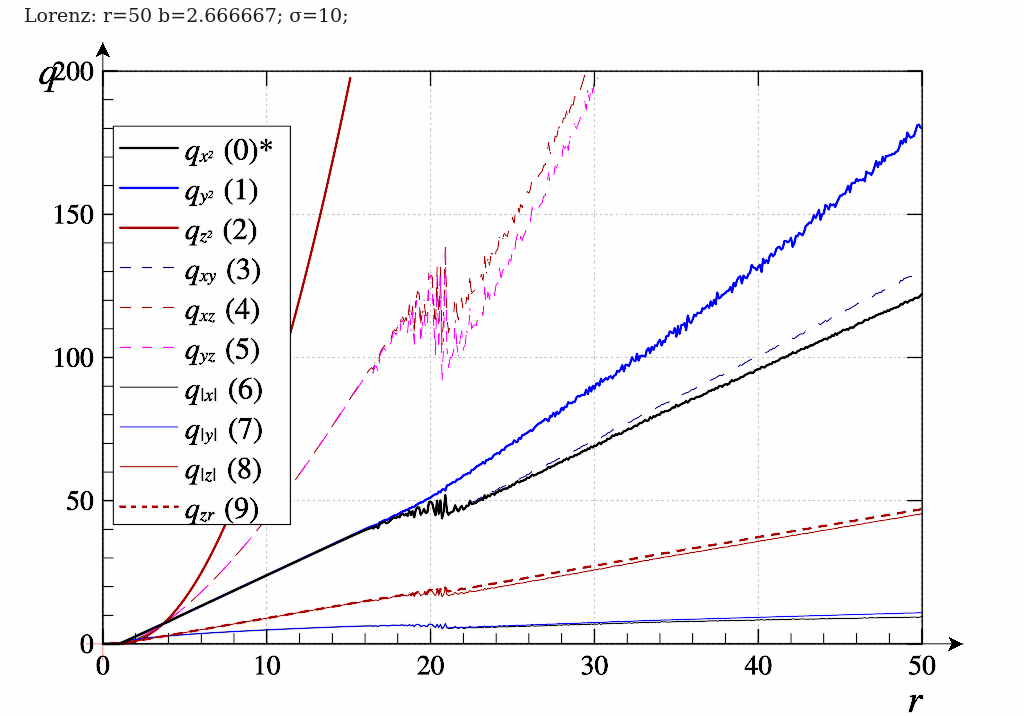
\includegraphics[width=0.7\textwidth]{../p5/p/cha/lor/lor_q-p_q_r.png}
    \caption{Розглянуті критерії для системи Лоренца}
    \label{atu:f:lor_q}
  \end{figure}

\end{frame}



% -----------------------------------------------------------------------

\begin{frame}
  \frametitle{}

  \Xhead{Система Лоренца: залежності критеріїв для двох параметрів}

\begin{figure}[htb!]
  \PicDouble{../p5/p/cha/lor/q2d/lor_qx2_r_b.png}{../p5/p/cha/lor/q2d/lor_qy2_r_b.png}
  \PicDoubleNL{../p5/p/cha/lor/q2d/lor_qz2_r_b.png}{../p5/p/cha/lor/q2d/lor_qxmy2_r_b.png}
  \vspace{-2.7ex}
  \begin{center}
    ~ \hfill c \hfill\hfill d \hfill ~
  \end{center}
  \vspace{-1.5ex}
  \caption{Залежності $q_{x^2}(r,b)$~(a), $q_{y^2}(r,b)$~(b), $q_{z^2}(r,b)$~(c), $q_{(x-y)^2}(r,b)$~(d) для системи Лоренца}
  \label{atu:f:lor_q_r_b}
\end{figure}

  Можлива одночасна ідентифікація параметрів
  $r$ і
  $b$, за умови спільного застосування критеріїв
  $q_{x^2}$ і
  $q_{z^2}$.

\end{frame}


% -----------------------------------------------------------------------

\begin{frame}
  \frametitle{}

  \Xhead{Система Sprott~A з додатковим параметром}

  \begin{equation}
    \begin{cases}
      \dot{x} =  c_{x_y} y, \\
      \dot{y} = -x + yz, \\
      \dot{z} =  1 - y^2.
    \end{cases}
    \label{atu:eq:spr_a}
  \end{equation}

Відмінною особливістю цієї системи є відсутність положень рівноваги, що унеможливлює
застосування багатьох відомих методів аналізу, заснованих на будь-якому
розкладі в околі точок рівноваги.

  \begin{figure}
    \PicDouble{../p5/p/cha/spr_a/sprott_a-p_xyz_cx_y=0x372.png}{../p5/p/cha/spr_a/sprott_a_f-p_f_cx_y=0x372.png}
    \caption{Аттрактор (a) та спектр (b) системи (\ref{atu:eq:spr_a}) при $c_{x_y} =0.372$}
    \label{atu:f:spr_a_p_0372}
  \end{figure}

  \begin{figure}[htb!]
    \PicDouble{../p5/p/cha/spr_a/sprott_a-p_xyz_cx_y=1x000.png}{../p5/p/cha/spr_a/sprott_a_f-p_f_cx_y=1x000.png}
    \caption{Аттрактор (a) та спектр (b) системи (\ref{atu:eq:spr_a}) при $c_{x_y} =1.0$}
    \label{atu:f:spr_a_p_1000}
  \end{figure}

\end{frame}

% -----------------------------------------------------------------------

\begin{frame}
  \frametitle{}

  \Xhead{}

\begin{figure}
  \begin{center}
    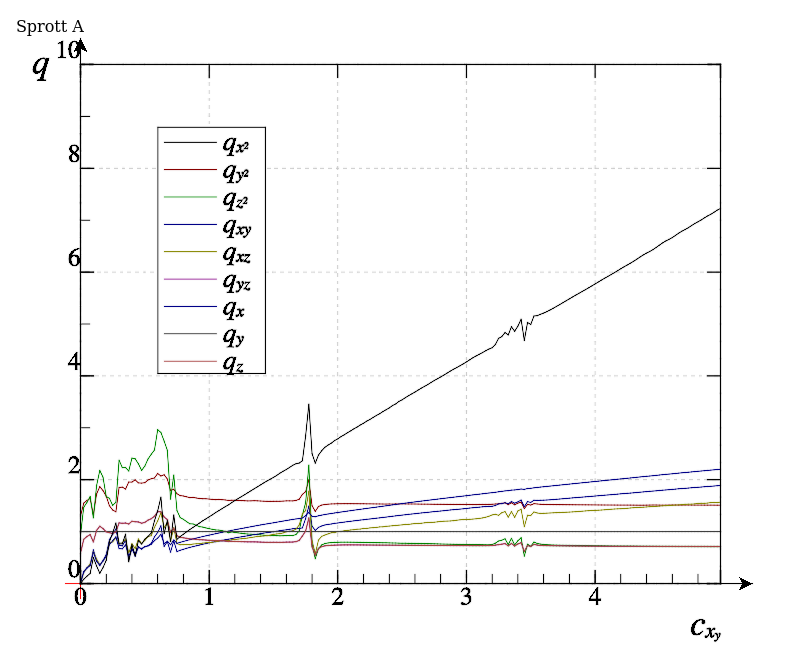
\includegraphics[width=0.60\textwidth]{../p5/p/cha/spr_a/sprott_a_q-p_c_x_y.png}
  \end{center}
  \caption{Залежності $q_{*}(c_{x_y})$ для системи (\ref{atu:eq:spr_a})}
  \label{atu:f:spr_a_q}
\end{figure}


\end{frame}





% -------------------------- P6 ---------------------------------------------


% -----------------------------------------------------------------------

\begin{frame}
  \frametitle{}

  \Xhead{}

  Програмно-апаратна складова комплексу реалізована на
  мікроконтролерах STM32 (ARM Cortex M4F). Використовувалася як власна
  розробка за базі STM32F407VE, так і отладочная плата на STM32F746ZI +
  допоміжні елементи.

  \begin{figure}[ht!]
    \centerline{\includegraphics[width=90\TW]{../p6/p/colp_stand.png} }
    \caption{Апаратно-програмний комплекс при роботі з генератором Колпітца}
    \label{atu:colp_stand}
  \end{figure}



\end{frame}


% -----------------------------------------------------------------------

\begin{frame}
  \frametitle{}
  %\framesubtitle{}
  \Xhead{Моделювання та ідентифікація фізичної системи пов'язаних релаксаційних генераторів}

  \begin{figure}
    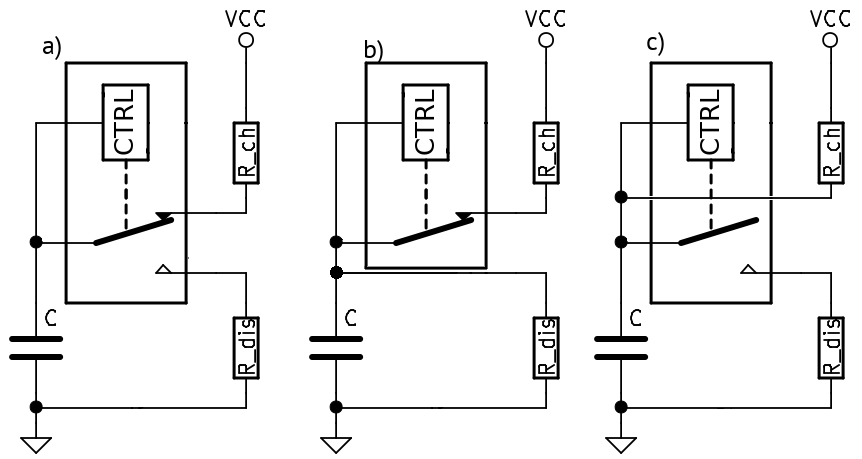
\includegraphics[width=0.68\textwidth]{../p7/p/relax_types.png}
    \caption{Умовні схеми релаксаційних генераторів}
  \end{figure}

\begin{equation}
  C \od{V_c}{t}
  =
  \frac{V\Tidx{cc} - V\Tidx{c}}{R\Tidx{ch}}
  - \frac{V\Tidx{c}}{R\Tidx{dis}} \cdot \mathrm{On}().
  \label{atu:eq:relax0}
\end{equation}

  \begin{figure}
    \centerline{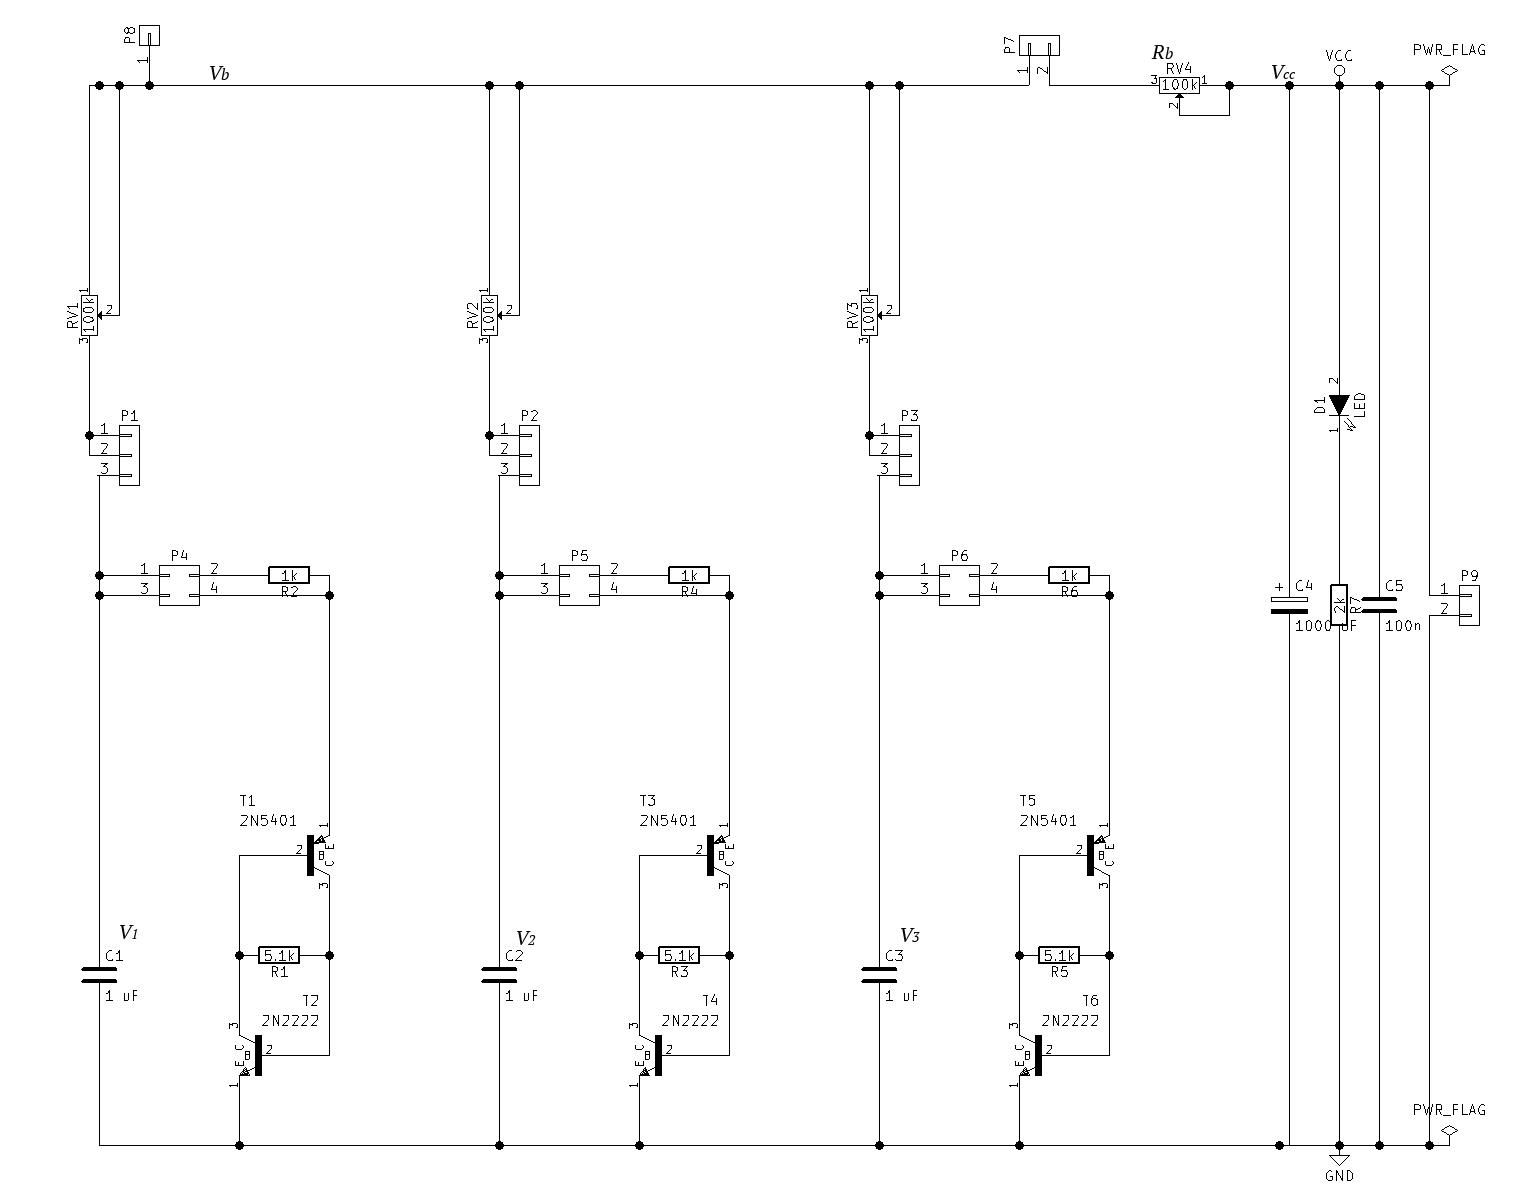
\includegraphics[width=0.86\textwidth]{../p7/p/relax3d_schem.png} }
    \caption{Електрична схема \RelaxBjtIi}
  \end{figure}


\end{frame}


% -----------------------------------------------------------------------

\begin{frame}
  \frametitle{}
  %\framesubtitle{}

  \Xhead{}

  \begin{figure}
    \PicDoubleS{../p7/p/relax3d_f_02.png}{../p7/p/relax3d_v1v2v3_02.png}
    \caption{Спектр $V_b(t)$~(a), і аттрактор~(b) для системи ``relax3d'' при $R_b = \SI{5.0}{\kilo \ohm} $}
    \label{atu:f:relax3d_f_02}
  \end{figure}

  \begin{figure}
    \PicDoubleS{../p7/p/relax3d_f_08.png}{../p7/p/relax3d_v1v2v3_08.png}
    \caption{Спектр $V_b(t)$~(a), і аттрактор~(b) для системи ``relax3d'' при $ R_b = \SI{34.0}{\kilo\ohm} $}
    \label{atu:f:relax3d_f_08}
  \end{figure}

  \begin{figure}
    \PicDoubleS{../p7/p/relax3d_f_09.png}{../p7/p/relax3d_v1v2v3_09.png}
    \caption{Спектр $V_b(t)$~(a), и аттрактор~(b) для системи ``relax3d'' при $R_b=\SI{36.0}{\kilo\ohm}$ }
    \label{atu:f:relax3d_f_09}
  \end{figure}

\end{frame}


% -----------------------------------------------------------------------

\begin{frame}
  \frametitle{}
  %\framesubtitle{}

  \Xhead{Модель систем з трьох пов'язаних релаксаційних генераторів}

  \begin{equation}
  \begin{cases}
    V_b = V_{cc} - R_b ( I_1 + I_2 + I_3 ), \\
      C_1 \dot{V}_1 = \frac{V_b-V_1}{R_{v1}} - \frac{V_1}{R_1} \mathrm{On}_1() - I_{1,\mathrm{leak}}(V_1), \\
      C_2 \dot{V}_2 = \frac{V_b-V_2}{R_{v2}} - \frac{V_2}{R_2} \mathrm{On}_2() - I_{2,\mathrm{leak}}(V_2), \\
      C_3 \dot{V}_3 = \frac{V_b-V_3}{R_{v3}} - \frac{V_3}{R_3} \mathrm{On}_3() - I_{3,\mathrm{leak}}(V_3), \\
      I_i = \frac{V_b-V_i}{R_{vi}}.
  \end{cases}.
    \label{atu:eq:relax3}
\end{equation}
%
де: \\
$R_b $ --- опір в ланцюзі живлення (ідентифікований параметр),
$C_i $ --- ємності кожного з релаксаційних генераторів,
$R_{vi} $ --- опори зарядки релаксаційних генераторів,
$R_{ i} $ --- опори зарядки релаксаційних генераторів,
$I_{i, \mathrm{leak}} $ --- струми витоку.


\end{frame}


% -----------------------------------------------------------------------

\begin{frame}
  \frametitle{}
  %\framesubtitle{}

  \Xhead{Критерії ідентифікації для системи ``relax3d''}

\begin{equation}
  q_{sv} = \overline{V_1+V_2+V_3} .
  \label{atu:eq:q_sv_relax}
\end{equation}
%
\begin{equation}
  q_{vb} = \overline{V_b} .
  \label{atu:eq:q_vb_relax}
\end{equation}
%
\begin{equation}
  q_{hv} = \frac{1}{\overline{V_b}} .
  \label{atu:eq:q_hb_relax}
\end{equation}
%
\begin{equation}
  q_{rv} = \frac{\overline{V_1+V_2+V_3}}{\overline{V_b}}.
  \label{atu:eq:q_rv_relax}
\end{equation}

  \begin{figure}
    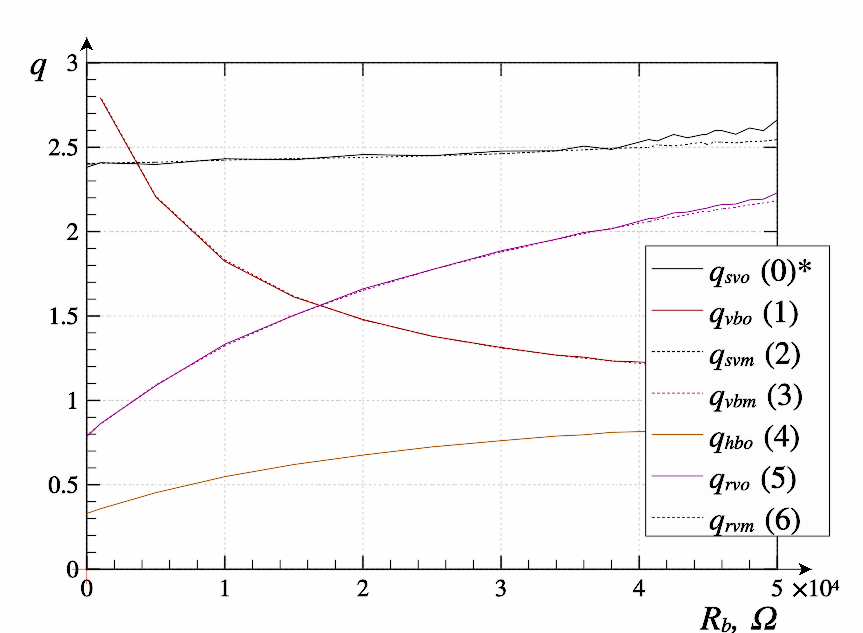
\includegraphics[width=0.7\textwidth]{../p7/p/relax3d_read_q-p_q1.png}
    \caption{Залежності для розглянутих критеріїв ідентифікації для системи релаксаційних генераторів на парі компліментарних транзисторів}
  \end{figure}


\end{frame}


% -----------------------------------------------------------------------

\begin{frame}
  \frametitle{}
  %\framesubtitle{}

  \Xhead{}

  \begin{figure}
    \PicDouble{../p7/p/relax3ds_read_id2_0-p_p.png}{../p7/p/relax3ds_read_id2_0-p_pp.png}
    \caption{Процес ідентифікації системи ``relax3ds'' групою методів ``Fq3zlovnAAF'': динаміка агентів~(a) та $p_\mathrm{id}$~(b)}
  \end{figure}

  \begin{figure}
    \PicDoubleNL{../p7/p/relax3ds_read_id2_prm_0-p_a_q.png}{../p7/p/relax3ds_read_id2_prm_0-p_q_gamma.png}
    \TextDouble{\caption{Залежності $\overline{e}_{r *}(a_q)$ при ідентифікації системи ``relax3ds''}}{\caption{Залежності $ \overline{e}_{r *} (q_\gamma) $ при ідентифікації системи ``relax3ds''}}
  \end{figure}


\end{frame}

% ----------------------------- FINAL ------------------------------------------

\begin{frame}
  \frametitle{Наукова новизна}
  %\framesubtitle{}

  \Xhead{Наукова новизна}

  \noindent
  \textbf{Вперше:}
  %
  \begin{itemize}

    \item
      створено критерії ідентифікації нелінійних динамічних систем,
      які, на відміну від тих, що існують, дозволяють оцінити їх стан та
      хаотичну динаміку, а також дають підстави для створення ефективних алгоритмів
      настроювання параметрів моделей систем ідентифікації;

    \item
      створено методи ідентифікації на підставі
      адаптивно-пошукової парадигми з використанням ансамблю пошукових агентів,
      які взаємодіють проміж собою, які на відміну від методів, що використовують
      одну модель або пару моделей, значно підвищують швидкість пошуку та
      здатні за мінімальний час  перелаштовуватися при різкій зміні параметрів, а на
      відміну від ройових алгоритмів нові методи потребують значно меншої
      кількості моделей та забезпечують певні гарантії пошуку;

    \item
      створено нову класифікацію систем ідентифікації динамічних систем,
      яка, як вбирає у себе методи, що існують, так і дозволяє
      створювати нові методи ідентифікації за рахунок
      комбінування їх складових частин;

    \item
      визначено, що системи з сухим тертям з точки зору задачі ідентифікації
      при певних  умовах функціонування
      мають властивості, що поєднують їх з системами хаотичної динаміки, тобто існує
      суттєва залежність від початкових
      умов та характерний вид атрактору;

    \item
      запропоновано модель системи хаотичної динаміки
      з використанням зв'язаних релаксаційних генераторів,
      яка відрізняється від існуючих відсутністю індуктивних компонентів,
      працездатністю при малих напругах та можливістю
      керування частотним діапазоном у широкому інтервалі,
      що сприяє процесу аналізу хаотичної динаміки
      фізичного об'єкту, перевірці адекватності математичної моделі
      та властивостей системи ідентифікації.
  \end{itemize}


\end{frame}




% -----------------------------------------------------------------------

\begin{frame}
  \frametitle{Практическая ценность}
  %\framesubtitle{}

  \noindent
  \textbf{ Набуло подальший розвиток:}
  \begin{itemize}

    \item
      методи оцінювання якості ідентифікації,
      які на відміну від тих, що існують,
      враховують використання множини агентів;

    \item
      підходи до адаптації параметрів систем
      ансамблевої ідентифікації, які придатні використовувати поточну
      інформацію від ансамблю синергірованих моделей та коригувати глобальні
      параметри пошуку в умовах апріорної та поточної невизначеності;

    \item
      модель генератора Колпітца, яка враховує
      більшу кількість нелінійних ефектів,
      що забезпечує більш адекватні результати процесу
      ідентифікації її параметрів запропонованими методами;
  \end{itemize}


\textbf{Практичне значення одержаних результатів.}
Розроблені методи ідентифікації було використано
при проектуванні, створенні, налаштовуванні параметрів
стенду дослідження вібраційного та акустичного впливу.
Аналіз результатів даних з цього стенду
дав можливість вказати необхідні нелінійні властивості системи
та діапазон параметрів, які у сукупності
забезпечують широкосмуговий спектр коливань.

Створене програмне середовище для моделювання нелінійних динамічних систем
використовується при проведенні практичних робіт по дисциплінам
``Моделювання систем'',
``Сучасні системи управління'' на кафедрі інформаційних технологій
і систем Національної металургійної академії України.

\end{frame}




% -----------------------------------------------------------------------

\begin{frame}
  \frametitle{}
  %\framesubtitle{}

  \Xhead{}


\end{frame}



% -----------------------------------------------------------------------

\begin{frame}
  \frametitle{Друковані роботи та апробація}
  %\framesubtitle{}

  \Xhead{Друковані роботи та апробація}

За темою дисертаційної роботи опубліковано
50 наукових праць. Основний зміст і результати досліджень
викладено у 36 друкованих працях у наукових фахових виданнях, які
рекомендовано Міністерством освіти і науки України,
29 --- включено до інших міжнародних наукометричних баз,
у тому числі 1 --- включено до бази Web of Science,
13 робіт опубліковано у збірниках наукових праць та матеріалах конференцій.

\smallskip

%{\scriptsize
Основные положения диссертационной работы докладывались на
научно-практических конференциях:
``Інформатика та системні науки'' (ІСН-2011) Полтава--2011,
``Интеллектуальные системы принятия решений и проблемы вычислительного интеллекта'' (ISDMCI) Херсон--2011,
``Информационные технологии в управлении сложными системами'' Днепропетровск--2011,
``Автоматизация: проблемы, идеи, решения'' Севастополь--2011,
``Интеллектуальные системы принятия решений и проблемы вычислительного интеллекта'' (ISDMCI) Херсон--2012,
``Автоматизация: проблемы, идеи, решения'' Севастополь--2012,
``Интеллектуальные системы принятия решений и проблемы вычислительного интеллекта'' (ISDMCI) Херсон--2013,
``Автоматизация: проблемы, идеи, решения'' Севастополь--2013,
``Интеллектуальные системы принятия решений и проблемы вычислительного интеллекта'' (ISDMCI) Херсон--2014,
``Интеллектуальные системы принятия решений и проблемы вычислительного интеллекта'' (ISDMCI) Херсон--2015,
``Computer Sciences and Information Technologies'' (CSIT) Lviv--2015 (Scopus),
``Интеллектуальные системы принятия решений и проблемы вычислительного интеллекта'' (ISDMCI) Херсон--2016,
``Data Stream Mining and Processing'' DSMP Lviv--2016 (Scopus,Web of Science).
%} % scriptsize

\end{frame}




% -----------------------------------------------------------------------

\begin{frame}
  \frametitle{Висновки}
  %\framesubtitle{}

  \Xhead{Висновки}

У роботі вирішена науково-технічна проблема ідентифікації параметрів складних технічних
систем у режимі хаотичної динаміки
з метою забезпечення їх керованої поведінки. При цьому:

\begin{itemize}

  \item
    створено нові критерії ідентифікації, які, на відміну від тих, що
    існують, придатні для аналізу стану та динаміки
    хаотичних систем, що створило фізично зумовлене обґрунтування працездатності систем
    ідентифікації;

  \item
    створено новий клас систем ідентифікації у межах
    адаптивно-пошуковой парадигми,
    які, за рахунок використання колективної динаміки
    ансамблю пошукових агентів, забезпечують
    кращу швидкість ідентифікації без істотного впливу на похибку ідентифікації;

  \item
    проведена перевірка працездатності запропонованих методів
    на прикладах як відомих систем хаотичної динаміки,
    так і на прикладах декількох інших динамічних систем (модельних та фізичних),
    які проявляють складну та хаотичну динаміку;

  \item
   визначено, що системи з сухим тертям з точки зору задачі ідентифікації
   при певних  умовах функціонування
   мають властивості, що поєднують їх з системами хаотичної динаміки;

 \item
  створено програмне забезпечення, придатне для моделювання як систем
  хаотичної динаміки, так і систем мультиагентної ідентифікації;

  \item
  проведено як комп'ютерне моделювання процесів ідентифікації систем
  хаотичної динаміки, так і фізичне моделювання таких, що підтверджує адекватність
  побудованих моделей.


\end{itemize}

\end{frame}



% -----------------------------------------------------------------------
%
% \begin{frame}
%   \frametitle{Выводы 2}
%   %\framesubtitle{}
%
%
% \end{frame}



\end{document}

